%% images/usecases.tex
%% Copyright (c) 2025 Enrico Stefanel <enrico.stefanel@studenti.units.it>


\documentclass{standalone}

\usepackage{tikz}
\tikzset{font=\sffamily}

% we want ER + above/below + left/right
\usetikzlibrary{er,positioning}

\usepackage{adjustbox}
\usetikzlibrary{shadows,positioning}

\begin{document}
\tikzset{
    every entity/.style = {top color=white,bottom color=blue!30},
    every attribute/.style = {top color=white, bottom color=yellow!20},
    every relationship/.style ={top color=white, bottom color=red!20},
}
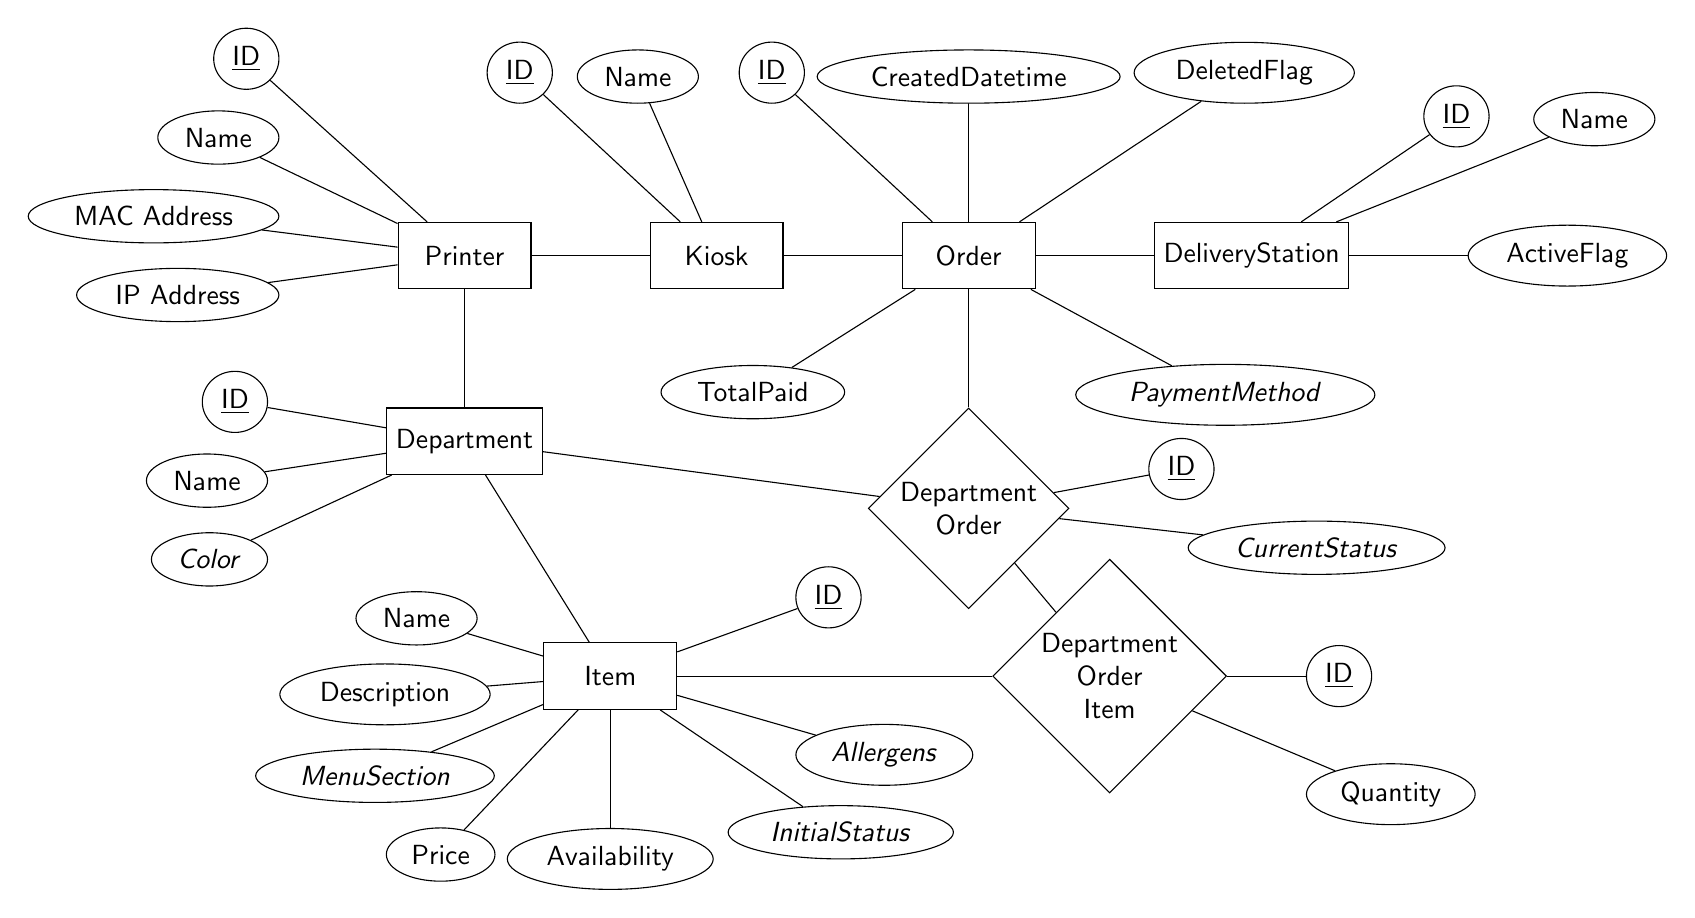
\begin{tikzpicture}[auto,node distance=1.5cm]
    \node[entity] (printer) {Printer};
    \node[attribute] (printer1) [left= of printer, yshift=2.5cm] {\underline{ID}} edge (printer);
    \node[attribute] (printer2) [left= of printer, yshift=1.5cm] {Name} edge (printer);
    \node[attribute] (printer2) [left= of printer, yshift=0.5cm] {MAC Address} edge (printer);
    \node[attribute] (printer2) [left= of printer, yshift=-0.5cm] {IP Address} edge (printer);

    \node[entity] (department) [below = of printer] {Department};
    \node[attribute] (department1) [left= of department, yshift=0.5cm] {\underline{ID}} edge (department);
    \node[attribute] (department2) [left= of department, yshift=-0.5cm] {Name} edge (department);
    \node[attribute] (department3) [left= of department, yshift=-1.5cm] {\textit{Color}} edge (department);

    \node[entity] (kiosk) [right = of printer] {Kiosk};
    \node[attribute] (kiosk1) [above= of kiosk, xshift=-2.5cm] {\underline{ID}} edge (kiosk);
    \node[attribute] (kiosk2) [above= of kiosk, xshift=-1cm] {Name} edge (kiosk);

    \node[entity] (order) [right = of kiosk] {Order};
    \node[attribute] (order1) [above = of order, xshift=-2.5cm] {\underline{ID}} edge (order);
    \node[attribute] (order2) [above = of order] {CreatedDatetime} edge (order);
    \node[attribute] (order3) [above = of order, xshift=3.5cm] {DeletedFlag} edge (order);
    \node[attribute] (order4) [below right = of order] {\textit{PaymentMethod}} edge (order);
    \node[attribute] (order5) [below left = of order] {TotalPaid} edge (order);

    \node[relationship] (department_order) [below = of order,align=center] {Department\\Order};
    \node[attribute] (department_order1) [right = of department_order,xshift=-0.5cm,yshift=0.5cm] {\underline{ID}} edge (department_order);
    \node[attribute] (department_order2) [right = of department_order,yshift=-0.5cm] {\textit{CurrentStatus}} edge (department_order);

    \node[entity] (delivery_station) [right = of order] {DeliveryStation};
    \node[attribute] (delivery_station1) [above right = of delivery_station] {\underline{ID}} edge (delivery_station);
    \node[attribute] (delivery_station1) [above right = of delivery_station, xshift=1.5cm] {Name} edge (delivery_station);
    \node[attribute] (delivery_station1) [right = of delivery_station] {ActiveFlag} edge (delivery_station);

    \node[entity] (item) [below left = of department_order, xshift=-2cm] {Item};
    \node[attribute] (item1) [right = of item,yshift=1cm] {\underline{ID}} edge (item);
    \node[attribute] (item2) [above left = of item,yshift=-1cm] {Name} edge (item);
    \node[attribute] (item3) [above left = of item,yshift=-2cm] {Description} edge (item);
    \node[attribute] (item4) [above left = of item,yshift=-3cm] {\textit{MenuSection}} edge (item);
    \node[attribute] (item5) [above left = of item,xshift=0.25cm,yshift=-4cm] {Price} edge (item);
    \node[attribute] (item6) [below = of item] {Availability} edge (item);
    \node[attribute] (item6) [below right = of item,yshift=-0.25cm] {\textit{InitialStatus}} edge (item);
    \node[attribute] (item6) [right = of item,yshift=-1cm] {\textit{Allergens}} edge (item);

    \node[relationship] (department_order_item) [right = of item,align=center,xshift=2.5cm] {Department\\Order\\Item};
    \node[attribute] (department_order_item1) [right = of department_order_item,xshift=-0.5cm] {\underline{ID}} edge (department_order_item);
    \node[attribute] (department_order_item2) [right = of department_order_item,xshift=-0.5cm,yshift=-1.5cm] {Quantity} edge (department_order_item);

    \path (kiosk) edge (order);
    \path (delivery_station) edge (order);
    \path (department) edge (printer);
    \path (kiosk) edge (printer);
    \path (department_order) edge (department) edge (order);
    \path (department) edge (item);
    \path (department_order_item)	edge (department_order) edge	 (item);
\end{tikzpicture}

\end{document}